\documentclass[a4paper, 12pt]{article}
\usepackage{geometry}
\geometry{a4paper,
total={170mm,257mm},left=2cm,right=2cm,
top=2cm,bottom=2cm}

\usepackage{mathtext}
\usepackage{amsmath}
\usepackage[T2A]{fontenc}
\usepackage[utf8]{inputenc}
\usepackage[english,russian]{babel}
\usepackage{graphicx, float}
\usepackage{tabularx, colortbl}
\usepackage{caption}
\captionsetup{labelsep=period}

\newcommand{\parag}[1]{\paragraph*{#1:}}
\DeclareSymbolFont{T2Aletters}{T2A}{cmr}{m}{it}
\newcounter{Points}
\setcounter{Points}{1}
\newcommand{\point}{\arabic{Points}. \addtocounter{Points}{1}}
\newcolumntype{C}{>{\centering\arraybackslash}X}

\author{Калинин Даниил, Б01-110}
\date{\today}
\title{Лабораторная работа 4.7.3. Изучение поляризованного света}

\begin{document}
\maketitle
\parindent=0cm

\parag {Цель работы}
ознакомиться с методами получения и анализа 
поляризованного света.

\parag {В работе используются}
оптическая скамья с осветителем,
зелёный светофильтр, два поляройда, чёрное зеркало, полированная
эбонитовая пластинка, стопа стеклянных пластинок, слюдяные пластинки
разной толщины, пластинки в $\frac{1}{4}$ и $\frac{1}{2}$ длины
волны, пластика в одну длину волны для зелёного света (пластинка
чувствительного света).

\parag {Теоритическая справка} ~\\
Методы получения линейно поляризованного света. Для получения 
линейно поляризованного света применяются специальные оптические 
приспособления - поляризаторы. Направление колебаний электрического
вектора в волне, прошедшей через поляризатор, называется разрешенным 
направлением поляризатора. Всякий поляризатор может быть использован
для исследования поляризованного света, т. е. в качестве анализатора.
Интенсивность I линейно поляризованного света после прохождения 
через анализатор зависит от угла, образованного плоскостью колебаний 
с разрешенным направлением анализатора:
\begin{equation}
    I = I_0 cos^2(\alpha)
    \label{eq:mallus}
\end{equation}

Соотношение \eqref{eq:mallus} носит название закона Малюса.
Опишем несколько способов получения плоскополяризованного света.
Отражение света от диэлектрической пластинки. Отраженный от диэлектрика
свет всегда частично поляризован. Степень поляризации света, отраженного
от диэлектрической пластинки в воздух, зависит от показателя 
преломления диэлектрика n и от угла падения i. Как следует из 
формул Френеля, полная поляризация отраженного света достигается
при падении под углом Брюстера, который определяется соотношением

\begin{equation*}
    tg(i) = n
\end{equation*}

В этом случае плоскость колебаний электрического вектора в отраженном 
свете перпендикулярна плоскости падения. Преломление света в 
стеклянной пластинке. Поскольку отраженный от диэлектрической 
пластинки свет оказывается частично (или даже полностью) 
поляризованным, проходящий свет также частично поляризуется. 
Преимущественное направление колебаний электрического вектора в 
прошедшем свете совпадает с плоскостью преломления луча. Максимальная
поляризация проходящего света достигается при падении под углом 
Брюстера. Для увеличения степени поляризации преломлённого света 
используют стопу стеклянных пластинок, расположенных под углом 
Брюстера к падающему свету. Преломление света в двоякопреломляющих 
кристаллах. Некоторые кристаллы обладают свойством двойного 
лучепреломления. Это связано с различием поляризуемости молекул 
в разных направлениях (диэлектрическая проницаемость $\varepsilon$ 
определяет показатель преломления среды n). Двоякопреломляющий 
кристалл называют одноосным, если в нём существует одно направление 
с экстремальным значением $\varepsilon$, а в других (перпендикулярных) 
направлениях значения $\varepsilon$ одинаковы (тензор диэлектрической 
проницаемости образует эллипсоид вращения). Направления вдоль осей 
эллипсоида называют главными, одно из них - c экстремальным значением 
$\varepsilon$ - оптической осью. Линейно поляризованная волна, в 
которой вектор E перпендикулярен оптической оси, называется 
обыкновенной; если же вектор E имеет проекцию на оптическую ось, это
необыкновенная волна. Показатели преломления этих волн обозначают
через $n_o$ (ординарная волна) и $n_e$ (экстраординарная).

\parag {Ход работы} ~\\

\begin{figure}[h]
    \centering
    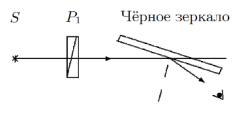
\includegraphics[scale=0.7]{pic_1.png}
    \caption{Определение разрешенных направлений черного зеркала}
    \label{img:pic_1}
\end{figure}

\point Размещяем на оптической скамье поляройд Р1 и чёрное зеркало, чтобы
плоскость падения была горизонтальна.

\point Поворачивая поляройд добиваемся наименьшей интенсивности отражённого
пятна. (Значения лимба на поляройде 10)

\point Фиксируя положение поляройда, вращаем зеркало, добиваемся минимальной
интенсивности.

\point Определяем разрешённое направление второго поляройда: устанавливаем
вместо черного зеркала второй поляройд и добиваемся минимальной 
интенсивности. (Значение на лимбе 2-го поляройда -8)

\point Устанавливаем вместо 2-го поляройда эбанитовое зеркало так,
чтобы го плоскось была перпендикулярна лучу(на глаз), отмечаем начало
отсчёта по лимбу (162).

\point Поворотом эбонитового зеркала, добиваемся минимальной интенсивности
записываем положение по лимбу (103).

\point Последние 2 измерения повторяем, установив светофильтр. Получим, соответственно, 162 и 106
(Эбонитовое зеркало люфтит на 2-3 градуса).

\point Рассичитываем показатель преллмления $n = tg(i)$, где $i = 59^\circ\pm3^\circ$. Получим: $tg(i) = 1.7\pm0.2$, относительная погрешность 12$\%$, табличное значение -- 1.6.

\begin{figure}[h]
    \centering
    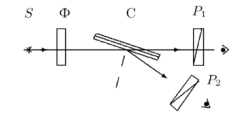
\includegraphics[scale=0.7]{pic_2.png}
    \caption{Исследование стопы}
    \label{img:pic_2}
\end{figure}

\point Вместо эбонитового зеркала выставляем стопу пластинок таким образом,
чтобы луч падал на неё под углом брюстера.

\point Вращая поляризаторы определяем характер полярризации света в
отражённом ($77^\circ$ от горизонтального направления т. е. вертикальная поляризация) и преломленном ($86^\circ$ от вертикального направления т. е. горизонтальная поляризация) 
лучах.

\begin{figure}[h]
    \centering
    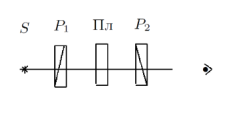
\includegraphics[scale=0.7]{pic_3.png}
    \caption{Определение главных направлений в пластинках}
    \label{img:pic_3}
\end{figure}

\point Устанавлиавем кристалическую однородную пластинку между поляройдами.
Вращая пластинку находим положения, когда главные направления пластинки
совпадают с разрешёнными направлениями поляройдов (значения на лимбе 88 и 0). 
Повторяем опыт для второй пластинки (Значения на лимбе 75 и -15).

\point Устанавливаем разрешённое направление 1-го поляройда горизонтально,
главные оси пластинки под углом $45^\circ$ к вертикали, устанавливаем световой фильтр.
Вращая 2-й фильтр устанавливаем поляризацию после прохождения пластинки по изменению цвета 
(1 - синий (линейная - $\lambda/2$), 2 - красный (круговая - $\lambda/4$))

\point Устанавливаем между поляройдами зелёный фильтр и пластинку чувствительного
оттенка. Устанавливаем разрешённое направление 1-го поляройда горизонтально
 и проверяем  с помощью 2-го поляройда, что пластинка не меняет поляризации
 зелёного света.

\point Убераем зелёный фильтр и убеждаемся, что стрелка имеет пурпурный
оттенок.

\begin{figure}[h]
    \centering
    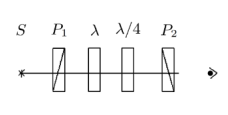
\includegraphics[scale=0.7]{pic_4.png}
    \caption{Определение направлений большей и меньшей скорости}
    \label{img:pic_4}
\end{figure}

\point Добавляем к схеме пластинку $\lambda / 4$, главные направления которой совпадают с главными направлениями "стрелки". При повороте пластинки на $180^\circ$ вокруг вертикальной оси цвет стрелки меняется с оранжевого (медленная ось) до голубого (быстрая ось).

\point Устанавливаем между полярйдами мозаичную пластинку, вращая пластинку
наблюдаем за изменениями цвета или интенсивности в отдельном квадратике.

\point Не трогая пластинку вращаем поляройд, следим за изменнениями. 
(При вращении пластинки угловые квадратики более заметно меняют интенсивность,
при вращении поляройда зветные угловые квадратикии меняются с крайними 
характеристеками).

\point Ставим зелёный фильтр, а за ним между скрещенными поляроидами - пластинку произвольной толщины ($\lambda$/4 с соседней установки).
Получаем эллиптически-поляризованный свет. Для этого устанавливаем
разрешённое направление первого поляроида под углом 10–20 к горизонтали 
так, чтобы вектор E падающего на пластинку света был расположен 
в первом квадранте. Установите разрешённое направление второго 
поляроида вертикально и, вращая пластинку, находим минимальную
интенсивность света, прошедшего второй поляроид. Вращая второй по-
ляроид, убеждаемся, что свет поляризован эллиптически, а не линейно
(в наборе есть пластинки $\lambda$/4 и $\lambda$/2). Получаем 
эллипс поляризации с вертикально ориентированной малой осью.
Для определения направления вращения светового вектора в эллипсе
установите между поляроидами дополнительную пластинку $\lambda$/4 с 
известными направлениями быстрой и медленной осей, ориентированными 
по осям эллипса поляризации анализируемого света. В этом
случае вектор E на выходе будет таким, как если бы свет прошёл две
пластинки $\lambda$/4: свет на выходе из второй пластинки будет линейно 
поляризован. Если пластинки поодиночке дают эллипсы, вращающиеся в
разные стороны, то поставленные друг за другом, они скомпенсируют
разность фаз, и вектор E на выходе останется в первом и третьем 
квадрантах. Если же световой вектор перешёл в смежные квадранты, значит,
эллипсы вращаются в одну сторону.

\parag {Заключение} ~\\
В ходе работы были определены разрешённые направления 2-х поляройдов,
рассчитан угол Бпрястера и показатель преломления для эбонита,
значение которого совпала с таблтчной в пределах погрешности. Также были изучены характеры поляризации
в отражённом и преломлённом лучах, найдены главные направления пластинок и направления большей
и меньшей скорости пластинок. Было определено направление вращения светового вектора в 
элептически поляризованной волне. Была изучен интерференция поляризованных
лучей.  

\end{document}
